\documentclass[letterpaper, 12 pt, conference]{ieeeconf}
\IEEEoverridecommandlockouts
\overrideIEEEmargins

%---------------- Letter Paper --------------------%
% be sure to change in document class too
\textwidth = 6.9 in
\textheight = 9.0 in
\oddsidemargin = -0.2 in
\evensidemargin = 0.0 in
\topmargin = -0.1 in
%\bottommargin = -0.5 in
\headheight = 0.0 in
\headsep = 0.25in
\parskip = 0.00in
\parindent = 0.1in

% The following packages can be found on http:\\www.ctan.org
\usepackage{graphics}
\usepackage{graphicx}
\usepackage{epsfig}
\usepackage{mathptmx}
\usepackage{times}
\usepackage{amsmath}
\usepackage{amssymb}
\usepackage{siunitx}
\usepackage{multirow}
\usepackage{booktabs}
\usepackage{longtable}
\usepackage{rotating}
\usepackage{textcomp}
\usepackage{bm}
\usepackage{fancyhdr}
\usepackage{comment}
\usepackage{subcaption}
\usepackage{hyperref}
\hypersetup{
    colorlinks=true,
    linkcolor=blue,
    filecolor=magenta,      
    urlcolor=cyan,
}

\begin{document}

\title{\LARGE \bf Ragin' Cajuns' Autonomous Vehicles for Coastal Preservation}


\author{\textbf{Coaches}:\\Joshua Vaughan$^{1}$ and Yasmeen Qudsi$^2$ \\% <-this % stops a space
\textbf{Members}:\\Nathan Madsen, Brennan Moeller, Joseph Stevens, and Benjamin Willis \\
\thanks{$^{1}$Department of Mechanical Engineering,
        University of Louisiana at Lafayette, Lafayette, LA 70504, USA
        {\tt\small joshua.vaughan@louisiana.edu}}%1
\thanks{$^{2}$Department of Mechanical Engineering,
        University of Louisiana at Lafayette, Lafayette, LA 70504, USA
        {\tt\small yasmeen.qudsi@louisiana.edu}}%        
}

\bibliographystyle{IEEEtran}
\pagestyle{fancyplain}
\lhead{\footnotesize{\textit{Ragin' Cajun RoboBoat}}}
\rhead{\footnotesize{\thepage}}
\cfoot{}


\maketitle
\thispagestyle{fancyplain}
%
\begin{abstract}
This report will discuss the proposal for the addition of an OAK-D camera and how this addition can improve the safety of autonomous surface vessels used to monitor wetlands like those found in Louisiana. The main benefit that this camera would bring to the Ragin' Cajuns' research would be increasing the efficiency of the autonomous system by reducing the processes being completed by the on-board computer. Thus increasing the computational power for safety features on the boat. This addition would improve the localization precision the surface vessel by enabling more sensors, such as LiDar, to be added with the same computational setup. The main tasks that need to be completed when monitoring the wetlands are creating a datum for the specific area and collecting data periodically for comparison. To aid in developing these types of systems, an autonomous surface vessel (ASV) was created to compete in RoboNation's RoboBoat competition in 2019. The computer network communicates with individual components via the Robot Operating System (ROS). The processing of the on-board peripherals are carried out by one NVIDIA Jetson TX1. This system has the ability to achieve much more with the integration of an OAK-D camera.
\end{abstract}

\section{Problem Statement}
The Ragin’ Cajuns' are currently in pursuit of safer and more efficient autonomous maritime systems, specifically, maritime systems that would be used to monitor wetlands like those commonly found in Louisiana. Such vessels release the burden of completing the dull and dangerous aspects of wetlands monitoring off the hands of scientists and engineers working on preservation. The OAK-D camera would aid in increasing the efficiency of an autonomous maritime system by managing the bulk of the image processing. In doing so, the burden of the system's on-board processors would be reduced, allowing a larger percentage of computational resources to be dedicated to tasks such as sensor processing, data collection, navigation, and operational safety. The OAK-D camera will also assist in monitoring many of the visual features that indicate coastal erosion. The improved systems can be used to increase sample collection and enable other menial tasks typically done by hand, thus reducing the time it takes to complete these monitoring tasks and increasing the overall power efficiency of the vessel. 

A system the Ragin' Cajun's are using to research into this problem is an autonomous surface vessel (ASV) that was created in 2019 as seen in Figure \ref{fig:RoboBoat}. 
%
\begin{figure}[tb]
\centering
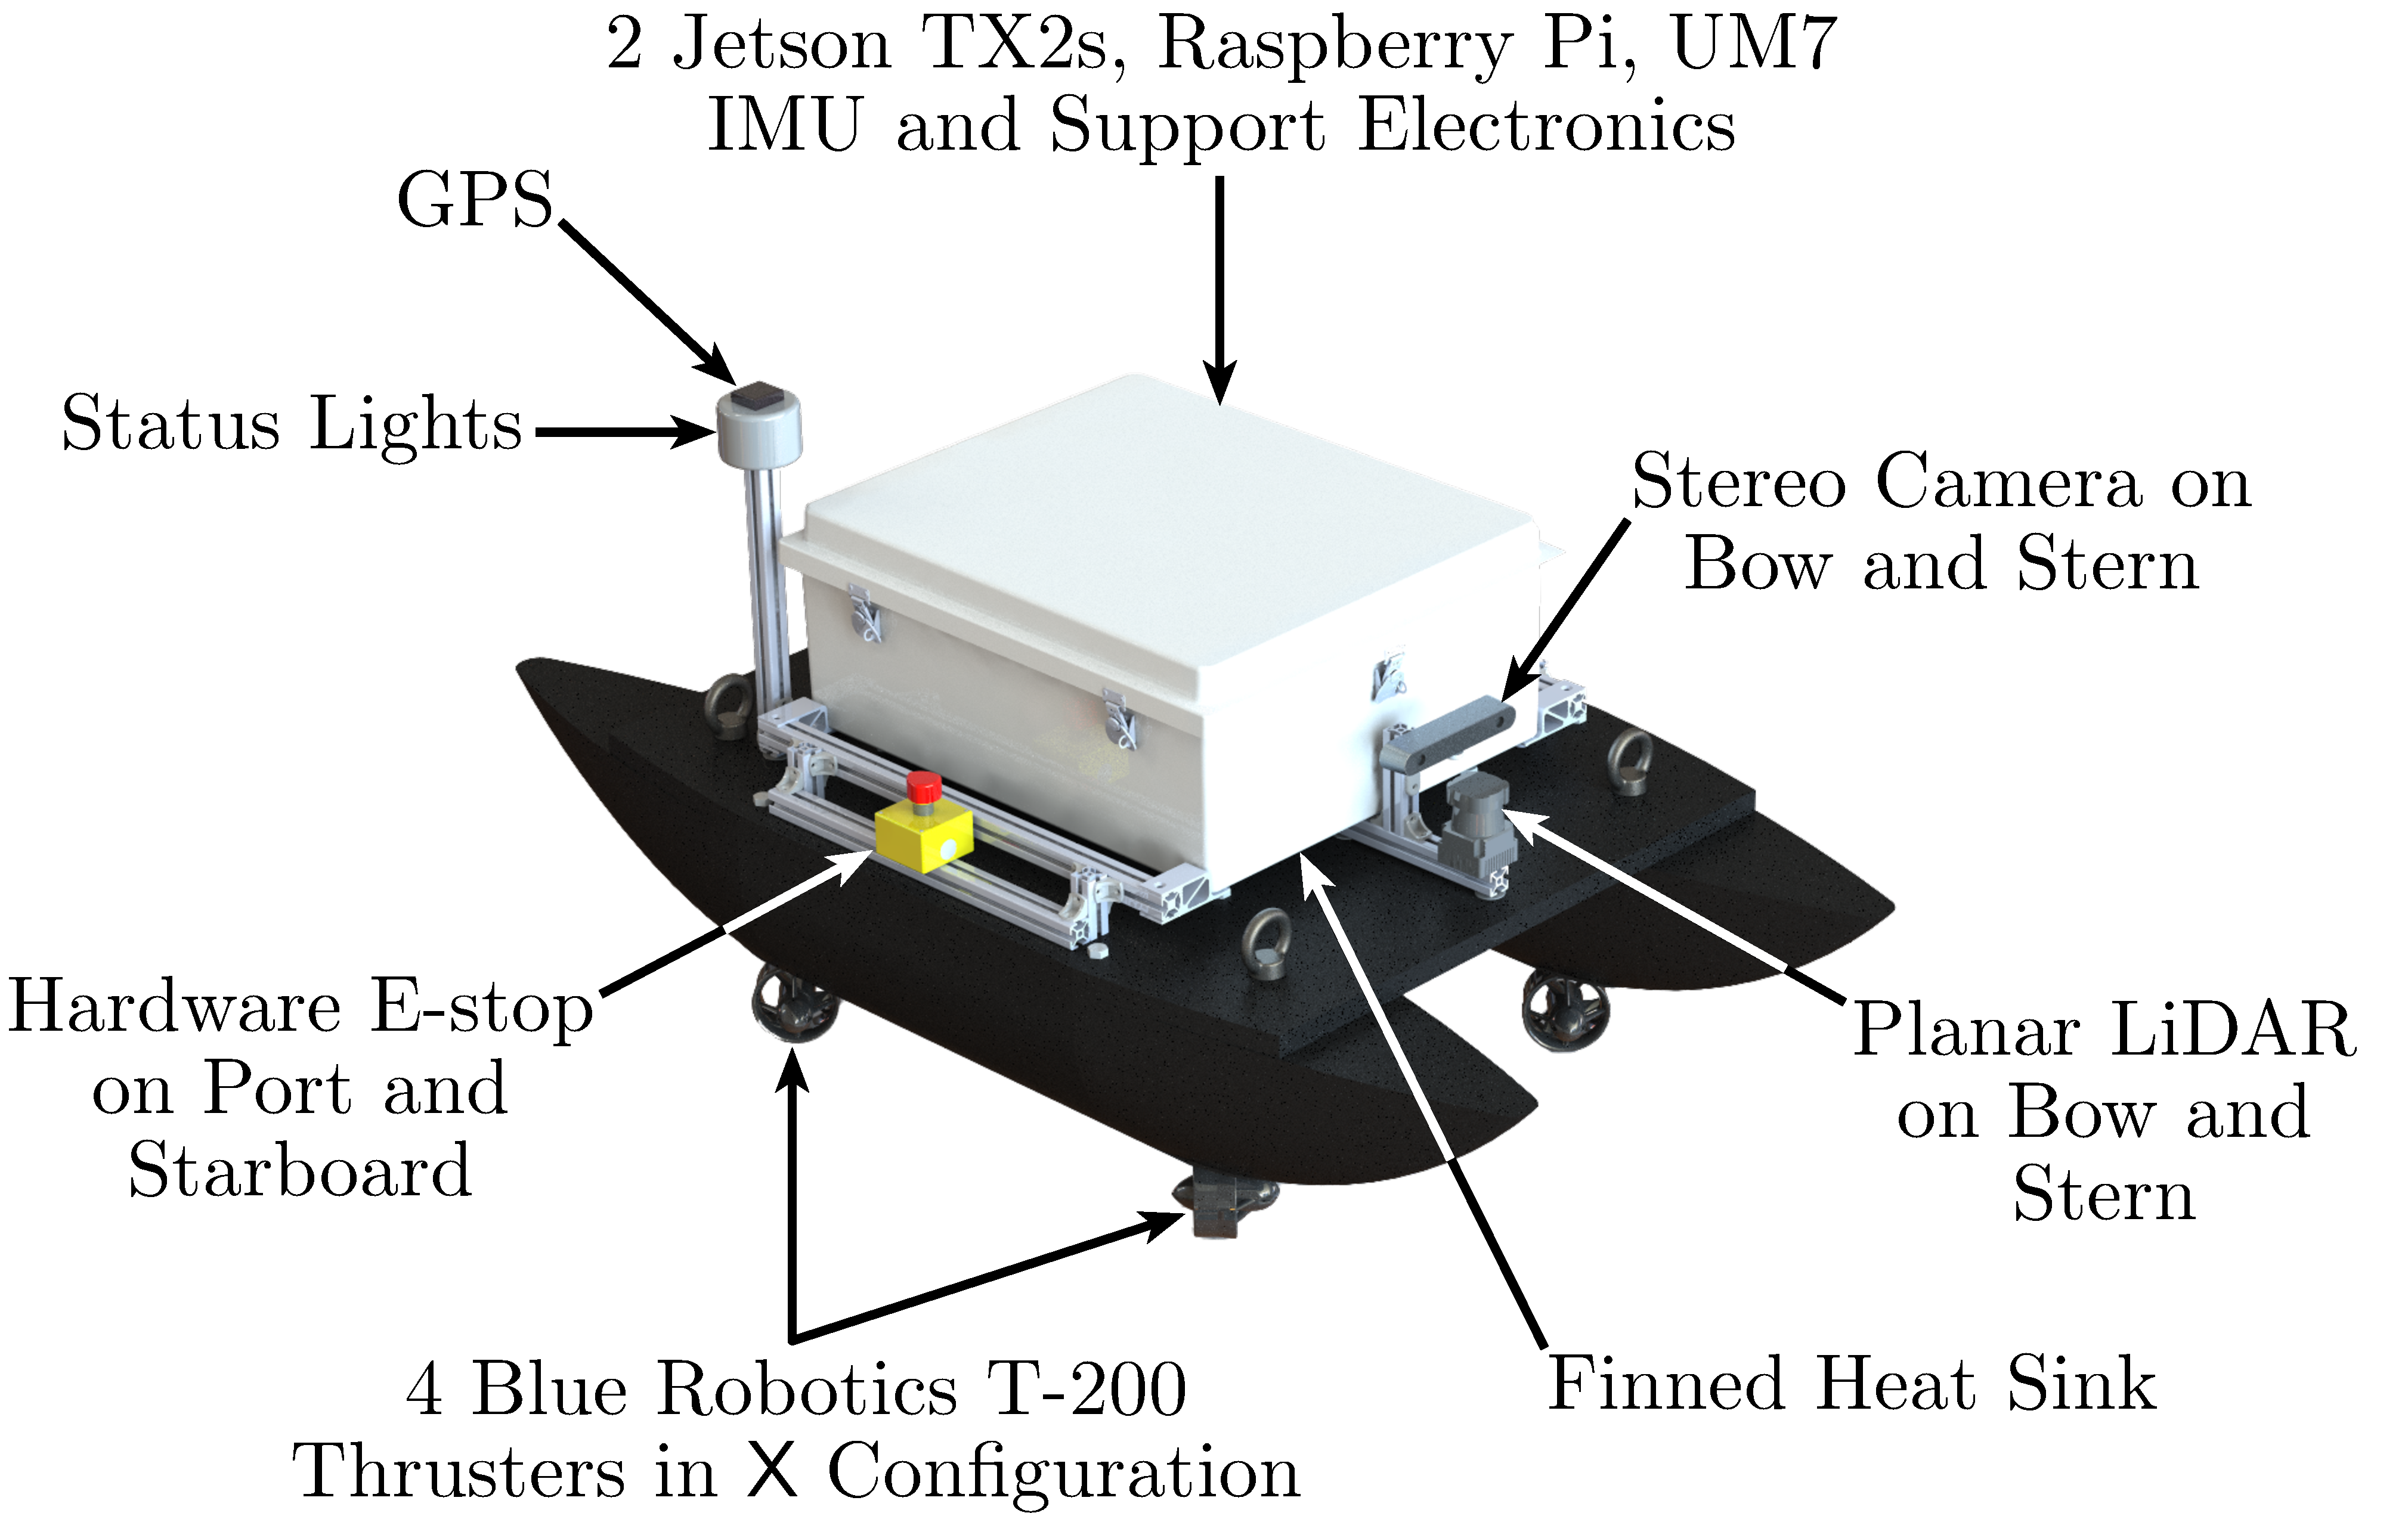
\includegraphics[width=\columnwidth]{Figures/Catamaran_Final_Render_3.pdf}
\caption{2020 Ragin' Cajuns RoboBoat CAD Model}
\label{fig:RoboBoat}
\end{figure}
%
This vessel attended the 2019 RoboNation RoboBoat competition where it won the \hyperlink{https://mechanical.louisiana.edu/news-events/news/20190627/university-team-earns-manufacturing-award-international-roboboat}{manufacturing award} for the hull’s design. The boat’s object detection algorithms have been in development since returning from the competition. 
In 2020, RoboNation held a virtual competition where the \hyperlink{https://crawlab.github.io/RoboBoat-2020/} {Ragin’ Cajuns} placed 2nd overall. The team was graciously featured on \hyperlink{https://clearpathrobotics.com/blog/2020/11/research-team-uses-clearpath-simulation-in-second-place-finish-at-roboboat-2020/}{Clearpath Robotics’ website} where the advancements that were made to the system by leveraging their systems for testing were publicized. In the ASV system, the OAK-D camera would be used to aid in the simultaneous localization and mapping (SLAM) of the RoboBoat course. The OAK-D’s data would be used in conjunction with RTK GPS and LiDAR data to aid in the localization precision. 
Another application of the OAK-D camera is on the unmanned aerial vehicle (UAV) that is currently being developed to integrate with maritime system for the 2021 RoboBoat competition. This camera would allow for the UAV to improve its autonomous flight by reducing the processing burden of the on-board computer to focus on sensor processing, data collection, and operational safety. Moreover, it would allow for the UAV to be more robust. This camera would create a larger computational budget by handling the post-processing normally computed on the on-board computer. This would enable more processing time to be spent on increasing the UAV’s ability to be versatile to new courses in the competition rather  than processing images, tracking objects, and classifying images. Due to weight constraints, most of the processing for the current visual peripherals must be carried out on the autonomous surface vessel. The OAK-D would replace one of the downward, visual peripherals and allow for the recognition and tracking of the buoys to be done by UAV. This would decrease the amount of processing being done on the autonomous surface vessel and allow for more processing to be spent on planning the best path through each course.
The RoboBoat competition would ensure that many of the same principles needed to aid scientist in coastal preservation be tested and iterated. The addition of the camera would give Ragin’ Cajuns the ability to improve the autonomous system for the RoboBoat competition, and more importantly, it would enable the Ragin’ Cajuns to work towards safer coastal preservation for wetlands like those found in Louisiana. This work would allow for the many scientist and engineers who work in this area to focus on more important tasks. 
\section{Team Capability} 
The members of this team are part of the \hyperlink{https://userweb.ucs.louisiana.edu/~jev9637/}{CRAWLAB} at the University of Louisiana at Lafayette. Research in the CRAWLAB ranges from vibration control of cranes and cable driven systems to industrial automation to mobile robotics. The foundation of this work is in conventional controls theory. However, recent work includes leveraging this conventional controls expertise with modern machine-learning-based methods. The overall aim is to reduce training times while improving the interpretability of the resulting models. These methods have been applied to both vibration control and gait design for walking robots.
Within the lab, machine-learning-based methods have been extensively used for perception and localization. For example, pipelines have been developed to identify buoys and other objects found in the \hyperlink{https://roboboat.org}{RoboBoat} and \hyperlink{https://robotx.org}{RobotX} contests, using ensembles of object detection models. This identification pipeline is in the process of being merged with other sensor data to improve the localization performance of the autonomous maritime systems on which it is deployed. 
In addition, there are many systems and hardware within the CRAWLAB to support the development and implementation of safe and efficient autonomous systems. There are two autonomous surface vessels (ASVs), a sixteen-foot WAM-V from Marine Advanced Research and a custom, smaller ASV. Work is currently in progress to integrate an unmanned aerial vehicle (UAV) with the smaller ASV. In addition, there is a GPU server with four TITAN XP GPUs to aid in training and evaluating the models developed through this project. **(Ms. Qudsi says "Needs more broad closing for the section". I was not sure where you wanted to go with this)**


\end{document}
